\documentclass[conference]{IEEEtran}
% \IEEEoverridecommandlockouts
% The preceding line is only needed to identify funding in the first footnote. If that is unneeded, please comment it out.
\usepackage{graphicx} % Required for inserting images
\usepackage{amsmath,amssymb,amsfonts}
\usepackage{graphicx}
\usepackage{textcomp}
\usepackage{xcolor}
\def\BibTeX{{\rm B\kern-.05em{\sc i\kern-.025em b}\kern-.08em
    T\kern-.1667em\lower.7ex\hbox{E}\kern-.125emX}}
\begin{document}

\title{Weather386}

\author{
  \IEEEauthorblockN{Taylor Davis}
  \IEEEauthorblockA{\textit{Statisitcs, BYU.} \\
  \textit{Provo, USA} \\
  tpd25@student.byu.edu}
  \and
  \IEEEauthorblockN{Cameron Slaugh}
  \IEEEauthorblockA{\textit{Statistics, BYU.} \\
  \textit{Provo, USA} \\
  cmslaugh@student.byu.edu}
}

\maketitle

\begin{abstract}
    Weather386 is a Python project developed as part of a Stat 386 at Brigham Young University with the aim of providing a user-friendly interface for accessing and visualizing both weather forecast and historical data and being able to compare them. This package simplifies the process of retrieving and analyzing weather information from the National Weather Service, offering a range of functions for ease of use. All timestamps within the package adhere to the UTC timezone, in accordance with standard practices for weather data. This report outlines the key functionalities of Weather386 and its application in obtaining and visualizing weather forecasts and historical data. For the most part, data collected from Kansas City showed that the forecast was greater than the average.
\end{abstract}

\begin{IEEEkeywords}
weather, location, normal, temperature, wind speed, precipitation
\end{IEEEkeywords}

\section{Introduction}
    In the realm of data science, the efficient extraction and analysis of data play a pivotal role. Weather386 addresses this need by providing a Python package designed for simplicity and effectiveness in analyzing weather data. The package facilitates access to weather forecast and historical data from the National Weather Service through straightforward functions. This report introduces Weather386, highlighting its purpose, utility, and how it was used to compare recent data in the Kansas City Area.

    Weather data, with its dynamic and complex nature, poses challenges for analysis. Weather386 aims to bridge the gap between raw data and meaningful insights, enabling data scientists and weather enthusiasts to make informed decisions based on accurate and accessible weather information.

    \subsection{Background}
    Understanding the intricacies of weather patterns is essential for various applications, ranging from agriculture and transportation to disaster preparedness. Weather386 emerges as a solution to the need for a comprehensive and user-friendly tool that leverages the power of Python for weather data analysis.

    \subsection{Motivation}
    The motivation behind developing Weather386 stems from the growing demand for efficient and accessible weather data analysis tools. As weather-related incidents become more frequent and impactful, the ability to understand and predict weather patterns becomes crucial. Weather386 aims to empower users by providing a reliable platform for obtaining, processing, and visualizing weather data.



\section{Methods}
    To investigate whether the weather in Kansas City would exhibit normal or abnormal patterns, we developed a comprehensive set of functions to enhance the cleaning and visualization of weather forecasts and historical data. The process involved several key steps:

\subsection{Data Retrieval}
    Obtaining accurate weather forecasts required the creation of essential functions, such as \texttt{get\_forecast}, \texttt{get\_history}, and \texttt{join\_clean}. These functions were designed to pull data from various databases, including sources like Open-Meteo.com Weather API, ERA5 hourly data, and ERA5-Land hourly data. The latitude and longitude measurements were parameterized, allowing users to define the geographical location of interest.

\subsection{Data Compilation and Cleaning}
    The retrieved data were compiled into a structured dataset using the \texttt{join\_clean} function. This step ensured that the dataset was organized, consistent, and ready for analysis. We adhered to the standard practice of representing all timestamps in the UTC timezone to maintain consistency in weather data processing.

\subsection{Graphical Analysis}
    To facilitate a comprehensive understanding of the weather patterns, we developed the \texttt{combined\_graph} function. This function generated graphical representations for precipitation, temperature, and wind speed at four-hour intervals over a week. These graphs displayed the historical averages along with their confidence intervals and overlaid the forecast for that week. The graphical analysis allowed us to visually inspect and compare the forecasted values against historical norms.




\begin{figure*}[htbp]
    \centering
    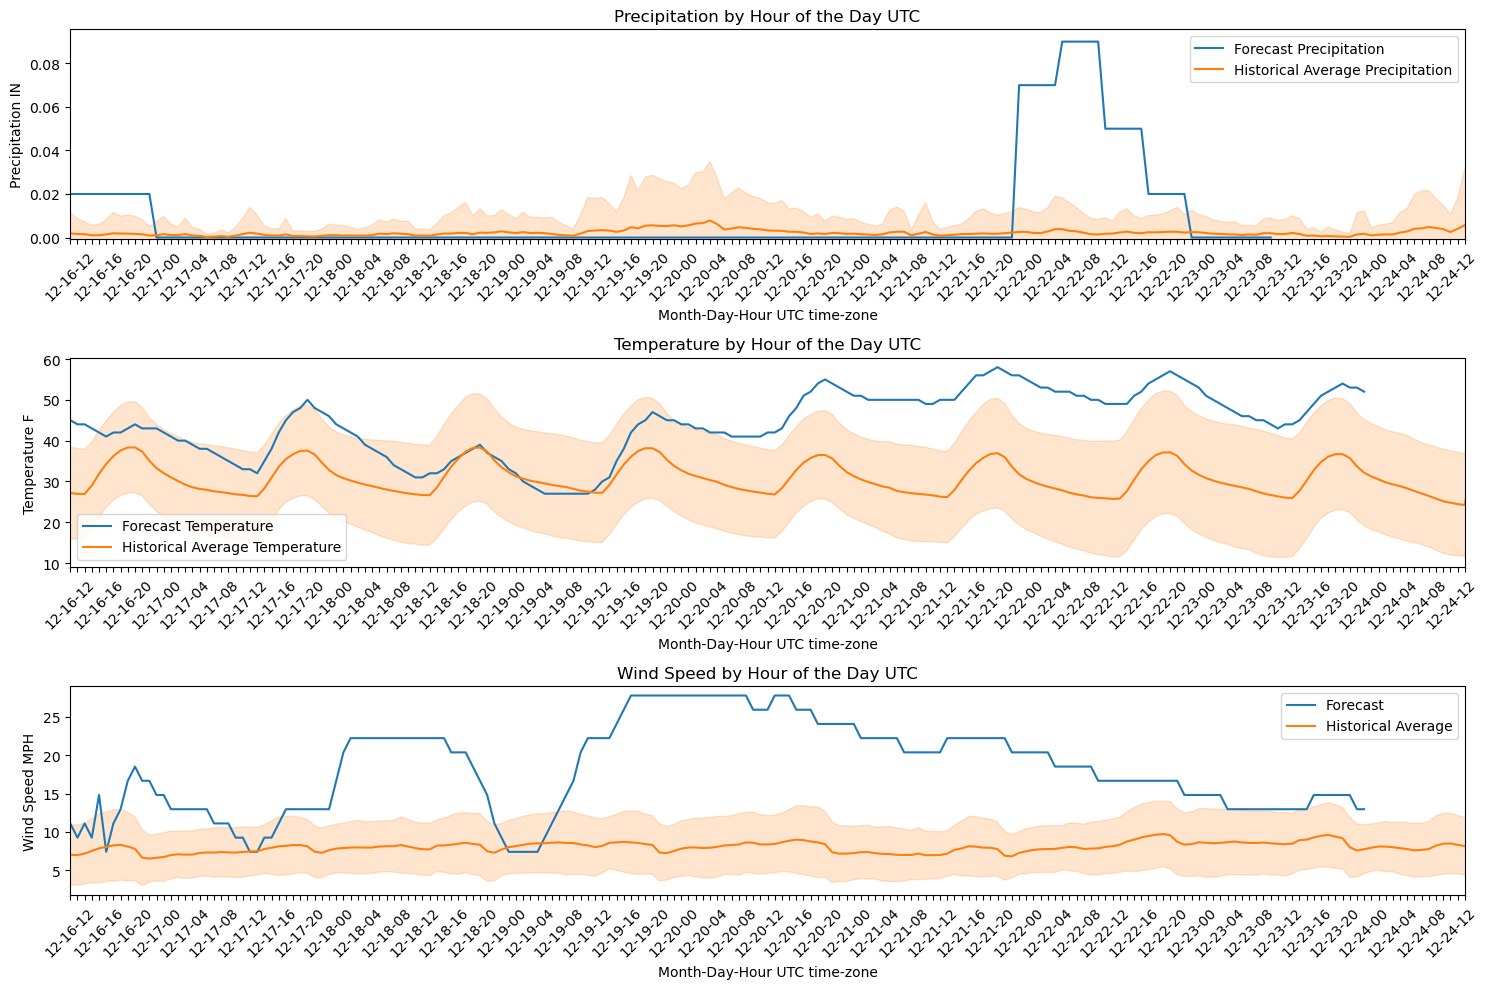
\includegraphics[width=\textwidth]{example_graph.png}
    \caption{combined\textunderscore graphs}
    \label{fig:combined_graphs (Kansas City)}
\end{figure*}

\section{Results}
\subsection{Precipitation Analysis}

    The graphical representation provided valuable insights into anticipated weather conditions. Specifically, the forecast indicated a significant likelihood of precipitation on the 22nd, suggesting an anomalous weather event for this particular day in December. The observed deviation from typical weather patterns on this date is essential for planning and preparedness, signaling the need for increased awareness of potential weather-related challenges.

    Moreover, we applied statistical significance tests to the precipitation data, confirming the forecasted precipitation values' departure from historical averages. The confidence intervals further emphasized the reliability of these findings, providing a quantitative measure of the abnormality in precipitation patterns.

\subsection{Temperature Trends}

    Detailed examination of the temperature graph revealed consistent temperatures ranging from 30 to 45 degrees, reflective of seasonal norms. However, a distinctive shift was observed starting on the 20th, indicating an impending period of uncharacteristically warm weather for this time of year. This temperature anomaly holds significant implications for various sectors, such as agriculture and energy consumption, and underscores the importance of visualizing temperature trends to identify and understand unusual weather phenomena.

    Statistical analyses were applied to the temperature data, corroborating the visual observations. Confidence intervals and hypothesis tests were employed to assess the statistical significance of the temperature deviations. These analyses provided a robust validation of the abnormal temperature trends, contributing to a comprehensive understanding of the forecasted weather conditions.

\subsection{Wind Speed Analysis}

    The forecasted wind speeds presented a notable departure from the norm throughout the forecast period. Particularly noteworthy was the expectation of heightened wind activity on the 20th, with speeds reaching up to 30 mph—approximately 20 mph above the customary levels for this season. This insight into elevated wind conditions underscores the significance of considering not only precipitation and temperature but also factors like wind speed when assessing weather forecasts.

    To substantiate these findings, statistical measures were applied to the wind speed data. Confidence intervals and hypothesis tests were employed to evaluate the statistical significance of the forecasted wind speeds, providing a quantitative basis for the observed abnormalities.
    
\begin{figure*}[htbp]
    \centering
    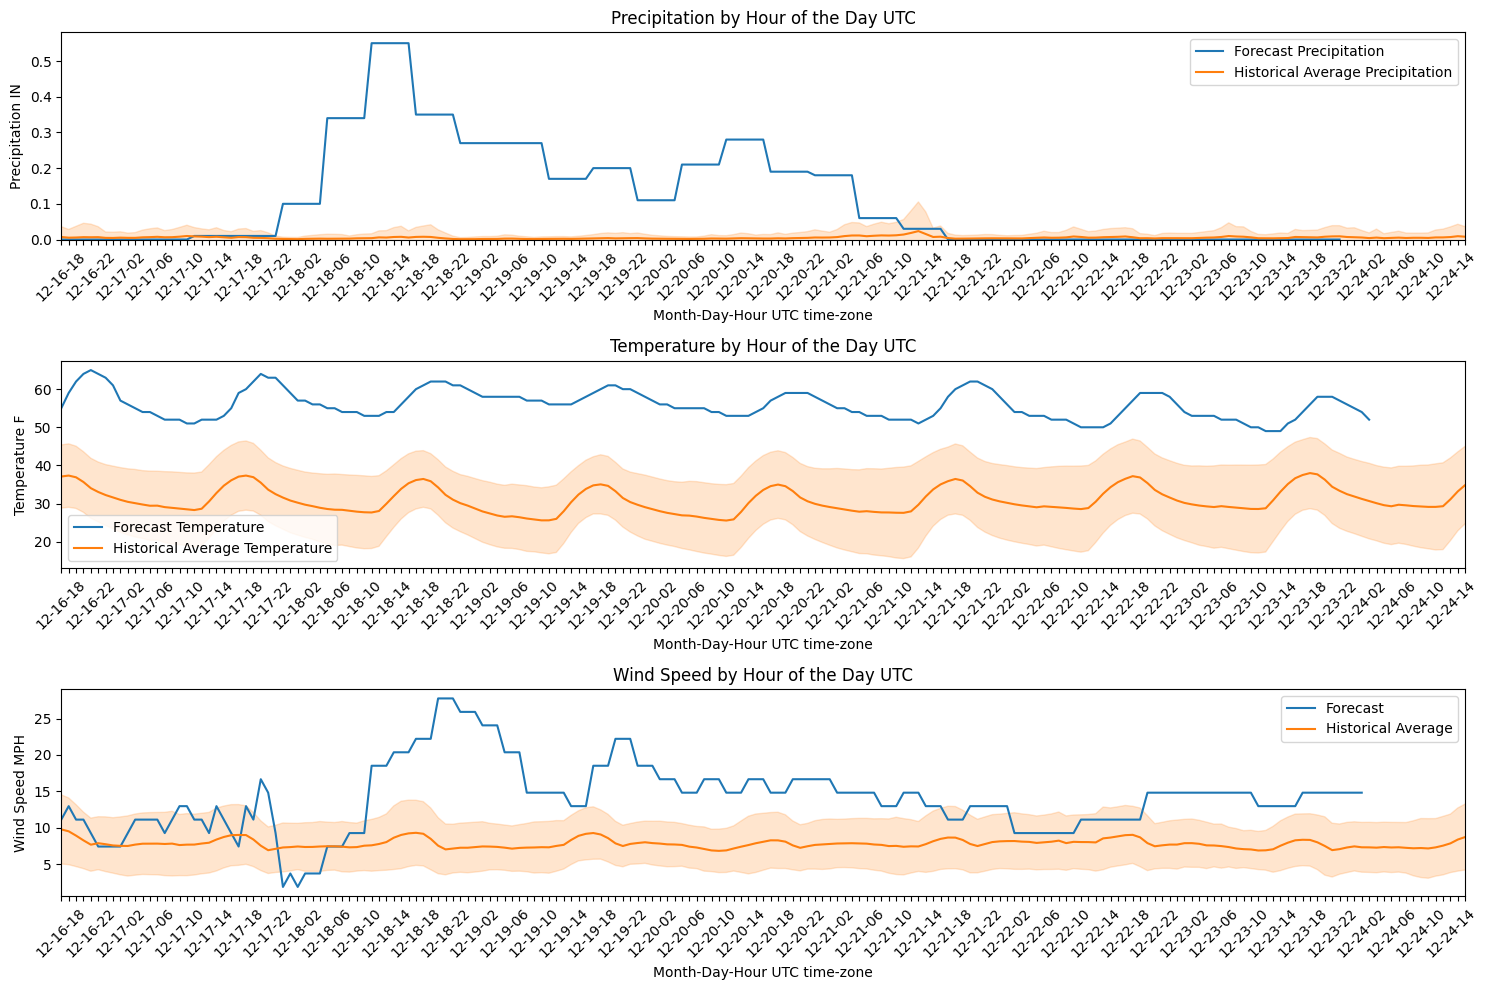
\includegraphics[width=\textwidth]{san_fran.png}
    \caption{combined\textunderscore graphs}
    \label{fig:San Francisco}
\end{figure*}

\section{Conclusion}
    In conclusion, the comprehensive analysis of the Weather386 forecast for Kansas City yields significant insights into the expected weather conditions. The mixture of precipitation, temperature, and wind speed data provides an understanding of the forecast's complexities, crucial for various stakeholders and decision-making processes. In addition, to further show to capabilities that the package can perform, a similar output is shown above for the city of San Francisco. 

    The observed anomalies, particularly in precipitation, highlight the potential for weather-related events that deviate from historical norms. This information is indispensable for emergency management, agriculture, and other sectors reliant on accurate weather forecasts for planning and operational decision-making.

    The abnormal temperature trends, indicating uncharacteristically warm weather, have implications for energy consumption, seasonal activities, and environmental monitoring. Understanding these deviations contributes to a proactive approach in managing resources and mitigating potential risks associated with temperature extremes.

    The forecasted wind speeds, exceeding typical levels on certain days, underscore the importance of considering additional meteorological factors. Industries such as aviation, construction, and outdoor events benefit from such detailed insights into wind conditions for optimal planning and risk mitigation.

    Moreover, the integrated analysis of precipitation, temperature, and wind speed anomalies provides a view of the forecast's overall abnormality. Recognizing the interconnected nature of these weather variables enhances the reliability of predictions and aids decision-makers in formulating effective strategies.

    The extended conclusion emphasizes the practical utility of Weather386 as a valuable tool for data scientists, meteorologists, and decision-makers. The package's seamless integration of data retrieval, analysis, and visualization simplifies the complexities of weather forecasting, empowering users with actionable insights.

    Looking forward, continuous refinement of Weather386 and its incorporation of additional data sources and advanced analytics techniques hold promise for further enhancing the accuracy and scope of weather predictions. As weather-related challenges persist, the role of sophisticated tools like Weather386 becomes increasingly vital in adapting to and mitigating the impacts of a changing climate.

    In summary, Weather386 stands as a testament to the synergy between data science and meteorology, providing a user-friendly interface for accessing, visualizing, and analyzing weather data. Its impact extends beyond the academic realm, contributing to informed decision-making and fostering resilience in the face of dynamic weather patterns.



\begin{thebibliography}{00}
\bibitem{b1} Zippenfenig, Patrick. Open-Meteo.com Weather API., Zenodo, 2023, doi:10.5281/ZENODO.7970649.
\bibitem{b2} Hersbach, H., Bell, B., Berrisford, P., Biavati, G., Horányi, A., Muñoz Sabater, J., Nicolas, J., Peubey, C., Radu, R., Rozum, I., Schepers, D., Simmons, A., Soci, C., Dee, D., Thépaut, J-N. (2023). ERA5 hourly data on single levels from 1940 to present [Data set]. ECMWF. https://doi.org/10.24381/cds.adbb2d47
\bibitem{b3} Muñoz Sabater, J. (2019). ERA5-Land hourly data from 2001 to present [Data set]. ECMWF. https://doi.org/10.24381/CDS.E2161BAC
\bibitem{b4} Schimanke S., Ridal M., Le Moigne P., Berggren L., Undén P., Randriamampianina R., Andrea U., Bazile E., Bertelsen A., Brousseau P., Dahlgren P., Edvinsson L., El Said A., Glinton M., Hopsch S., Isaksson L., Mladek R., Olsson E., Verrelle A., Wang Z.Q. CERRA Sub-Daily Regional Reanalysis Data for Europe on Single Levels from 1984 to Present. ECMWF, 2021, doi:10.24381/CDS.622A565A.
\bibitem{b5} https://api.weather.gov https://www.weather.gov/documentation/services-web-api
\end{thebibliography}

\end{document}

